\section{Preventivo}

Verranno utilizzate le seguenti abbreviazioni per indicare i ruoli:
\begin{itemize}
	\item \textbf{RE:} Responsabile
	\item \textbf{AM:} Amministratore
	\item \textbf{AN:} Analista
	\item \textbf{PT:} Progettista
	\item \textbf{PR:} Programmatore
	\item \textbf{VE:} Verificatore
\end{itemize}

Tenners applica le seguenti tariffe per tipo di ruolo coinvolto nell'attività di sviluppo:
\\
\begin{center}
\begin{tabular}{ |c|c|  }
 \hline
 Ruolo 		& Tariffa (EUR)\\
 \hline\hline
	Responsabile	& 30\\
	Amministratore	& 20\\
	Analista		& 25\\
	Progettista		& 22\\
	Programmatore	& 15\\
	Verificatore	& 15\\
 \hline
\end{tabular}
\end{center}
\newpage
\subsection{Fase di Analisi}
\subsubsection{Prospetto orario}
Il team ha previsto la seguente spartizione di ruoli per questa fase del progetto:
\\
\begin{center}
\begin{tabular}{ |c|c|c|c|c|c|c|c|  }
 \hline
 Membro 		& RE 	& AM 	& AN 	& PT 	& PR 	& VE 	& Tot.\\
 \hline\hline
 Simone			& 4 		& 8		& 12 	& 2 		& 0 		& 4 		& 30\\
 Gabriel		& 3 		& 2 		& 20 	& 2 		& 0 		& 3 		& 30\\
 Nicola			& 6 		& 0 		& 12 	& 0 		& 0 		& 12 	& 30\\
 Gianmarco		& 0 		& 2 		& 16 	& 2 		& 0 		& 10 	& 30\\
 Gezim			& 6 		& 10 	& 6 	& 2 		& 0 		& 6	 	& 30\\
 Paola			& 6 		& 2 		& 10 	& 2 		& 0 		& 10 	& 30\\
 Giovanni		& 6 		& 11 	& 8 	& 0 		& 0 		& 5  	& 30\\
 \hline\hline
 Ore totali		& 31		& 35		& 84 	& 10 	& 0 		& 50 	& 210\\
  \hline
\end{tabular}
\end{center}

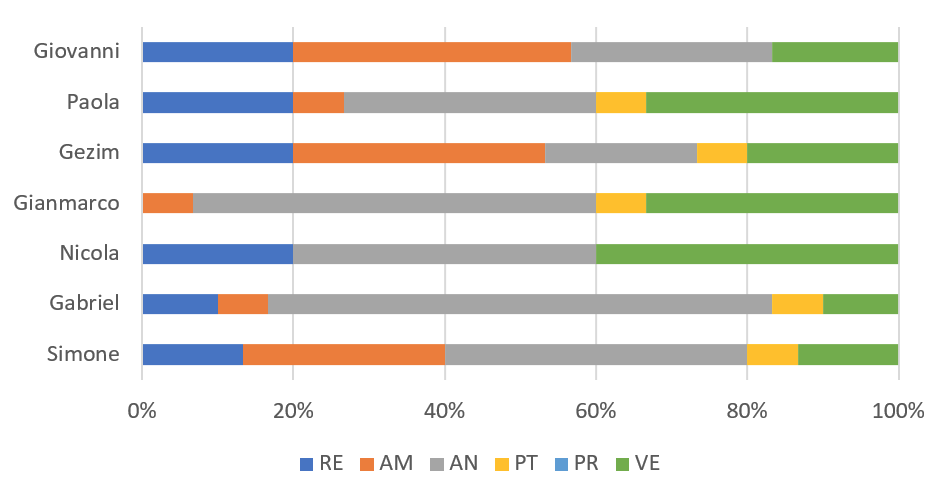
\includegraphics[width=\textwidth]{res/img/h12}

\subsubsection{Prospetto economico}
In abase alle ore necessarie per il completamento di questa fase, il valore economico totale è di 4.700,00 EUR.
\begin{center}
\begin{tabular}{ |c|c|c|  }
 \hline
 Ruolo 		& Ammontare ore 	& Totale (EUR)\\
 	\hline
 \hline
 	Responsabile	& 31 	& 930\\
	Amministratore	& 35		& 700\\
	Analista		& 84 	& 2100\\
	Progettista		& 10		& 220\\
	Programmatore	& 0		& 0\\
	Verificatore	& 50		& 750\\
 \hline\hline
 TOTALE		& 210		& 4700\\
  \hline
\end{tabular}
\end{center}
\newpage
\subsection{Fase di Presentazione}
\subsubsection{Prospetto orario}
Il team ha previsto la seguente spartizione di ruoli per questa fase del progetto:
\\
\begin{center}
\begin{tabular}{ |c|c|c|c|c|c|c|c|  }
 \hline
 Membro 		& RE 	& AM 	& AN 	& PT 	& PR 	& VE 	& Tot.\\
 \hline\hline
 Simone			& 0 		& 0		& 3 	& 0 		& 0 		& 2 		& 5\\
 Gabriel		& 0 		& 0 		& 2 	& 0 		& 0 		& 3 		& 5\\
 Nicola			& 0 		& 4 		& 1 	& 0 		& 0 		& 0 		& 5\\
 Gianmarco		& 3 		& 0 		& 2 	& 0 		& 0 		& 0 		& 5\\
 Gezim			& 0 		& 0 		& 2 	& 0 		& 0 		& 3	 	& 5\\
 Paola			& 0 		& 0 		& 5 	& 0 		& 0 		& 0 		& 5\\
 Giovanni		& 0 		& 0	 	& 3 	& 0 		& 0 		& 2  	& 5\\
 \hline\hline
 Ore totali		& 3		& 4		& 18 	& 0	 	& 0 		& 10 		& 35\\
  \hline
\end{tabular}
\end{center}

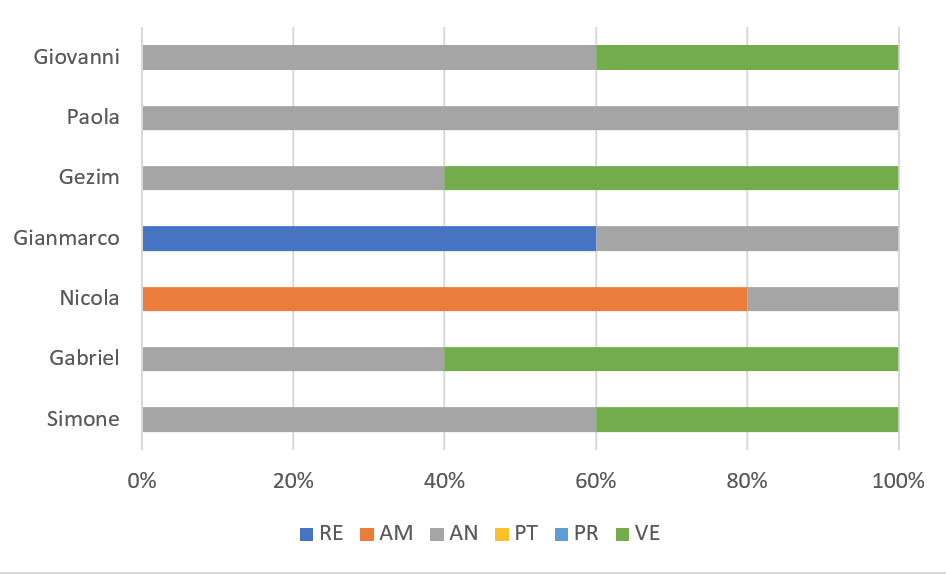
\includegraphics[width=\textwidth]{res/img/hi2}
\newpage
\subsubsection{Prospetto economico}
In abase alle ore necessarie per il completamento di questa fase, il valore economico totale è di 770,00 EUR.
\begin{center}
\begin{tabular}{ |c|c|c|  }
 \hline
 Ruolo 		& Ammontare ore 	& Totale (EUR)\\
 	\hline
 \hline
 	Responsabile	& 3 		& 90\\
	Amministratore	& 4		& 80\\
	Analista		& 18 	& 450\\
	Progettista		& 10		& 0\\
	Programmatore	& 0		& 0\\
	Verificatore	& 10		& 150\\
 \hline\hline
 TOTALE		& 35		& 770\\
  \hline
\end{tabular}
\end{center}
\newpage
\subsection{Fase di Progettazione Architetturale}
\subsubsection{Prospetto orario}
Il team ha previsto la seguente spartizione di ruoli per questa fase del progetto:
\\
\begin{center}
\begin{tabular}{ |c|c|c|c|c|c|c|c|  }
 \hline
 Membro 		& RE 	& AM 	& AN 	& PT 	& PR 	& VE 	& Tot.\\
 \hline\hline
 Simone			& 5 		& 0		& 6 	& 10 	& 4 		& 0 		& 25\\
 Gabriel		& 0 		& 5 		& 0 	& 12		& 8 		& 0 		& 25\\
 Nicola			& 0 		& 2 		& 0 	& 5 		& 5 		& 8 		& 25\\
 Gianmarco		& 5 		& 8 		& 0 	& 10 	& 0 		& 2 		& 25\\
 Gezim			& 0 		& 0 		& 10 	& 5 		& 4 		& 6	 	& 25\\
 Paola			& 0 		& 4 		& 6 	& 9 		& 0 		& 6 		& 25\\
 Giovanni		& 0 		& 0	 	& 5 	& 5 		& 5 		& 10  	& 25\\
 \hline\hline
 Ore totali		& 10		& 19		& 27 	& 56	 	& 26 	& 32 	& 170\\
  \hline
\end{tabular}
\end{center}

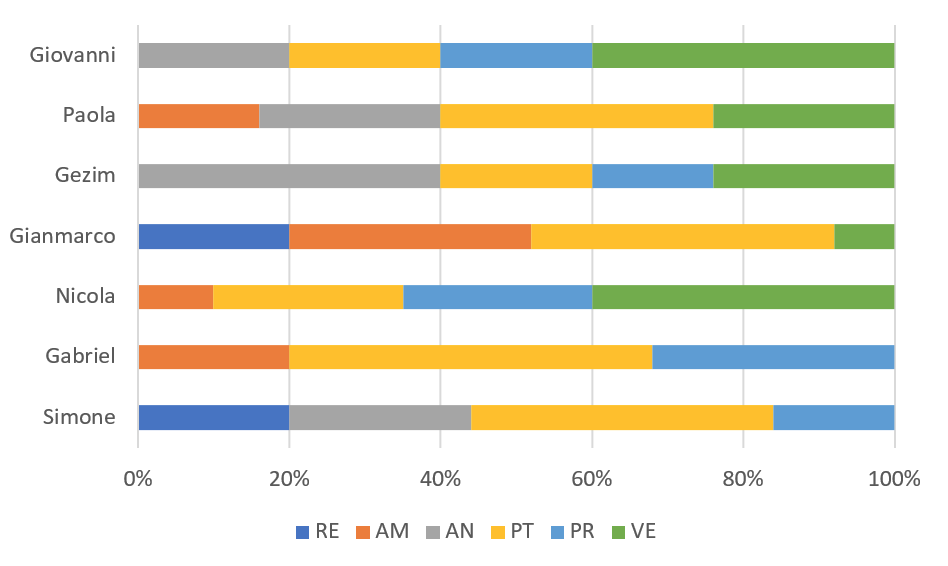
\includegraphics[width=\textwidth]{res/img/hi33}

\subsubsection{Prospetto economico}
In abase alle ore necessarie per il completamento di questa fase, il valore economico totale è di 3.847,00 EUR.
\begin{center}
\begin{tabular}{ |c|c|c|  }
 \hline
 Ruolo 		& Ammontare ore 	& Totale (EUR)\\
 	\hline
 \hline
 	Responsabile	& 10 		& 300\\
	Amministratore	& 19		& 380\\
	Analista		& 27 	& 675\\
	Progettista		& 56		& 1232\\
	Programmatore	& 26		& 780\\
	Verificatore	& 32 	& 480\\
 \hline\hline
 TOTALE		& 170		& 3847\\
  \hline
\end{tabular}
\end{center}

\newpage
\subsection{Fase di Progettazione di dettaglio e codifica}
\subsubsection{Prospetto orario}
Il team ha previsto la seguente spartizione di ruoli per questa fase del progetto:
\\
\begin{center}
\begin{tabular}{ |c|c|c|c|c|c|c|c|  }
 \hline
 Membro 		& RE 	& AM 	& AN 	& PT 	& PR 	& VE 	& Tot.\\
 \hline\hline
 Simone			& 0 		& 8		& 2 	& 10 	& 25 		& 10 		& 55\\
 Gabriel		& 5 		& 0 		& 0 	& 10		& 30 		& 10 		& 55\\
 Nicola			& 5 		& 8 		& 3 	& 9 		& 20 		& 10 		& 55\\
 Gianmarco		& 0 		& 0 		& 0 	& 15 	& 30 		& 10 		& 55\\
 Gezim			& 5 		& 6 		& 0 	& 12 		& 24 		& 8	 	& 55\\
 Paola			& 5 		& 2 		& 3 	& 15 		& 20 		& 10 		& 55\\
 Giovanni		& 5 		& 6	 	& 0 	& 10 		& 24 		& 10  	& 55\\
 \hline\hline
 Ore totali		& 25		& 30		& 8 	& 81	 	& 173 	& 68 	& 385\\
  \hline
\end{tabular}
\end{center}

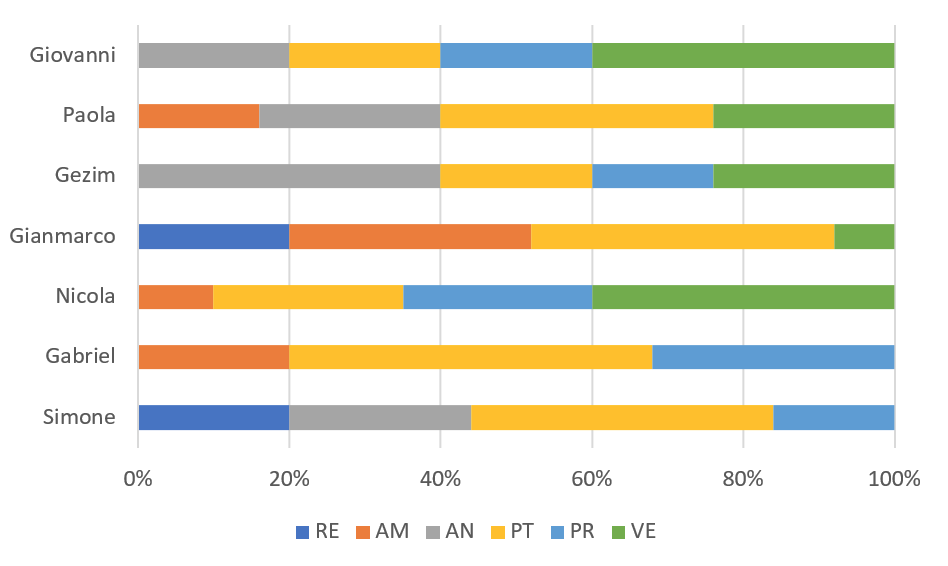
\includegraphics[width=\textwidth]{res/img/hi33}
\
\subsubsection{Prospetto economico}
In abase alle ore necessarie per il completamento di questa fase, il valore economico totale è di 9.542,00 EUR.
\begin{center}
\begin{tabular}{ |c|c|c|  }
 \hline
 Ruolo 		& Ammontare ore 	& Totale (EUR)\\
 	\hline
 \hline
 	Responsabile	& 25 		& 750\\
	Amministratore	& 30		& 600\\
	Analista		& 8 	& 200\\
	Progettista		& 81		& 1782\\
	Programmatore	& 173		& 5190\\
	Verificatore	& 68 	& 1020\\
 \hline\hline
 TOTALE		& 385		& 9542\\
  \hline
\end{tabular}
\end{center}

\newpage
\subsection{Fase di Validazione e Collaudo}
\subsubsection{Prospetto orario}
Il team ha previsto la seguente spartizione di ruoli per questa fase del progetto:
\\
\begin{center}
\begin{tabular}{ |c|c|c|c|c|c|c|c|  }
 \hline
 Membro 		& RE 	& AM 	& AN 	& PT 	& PR 	& VE 	& Tot.\\
 \hline\hline
 Simone			& 4 		& 0		& 0 	& 2 		& 4 		& 10 		& 20\\
 Gabriel		& 0 		& 6 		& 0 	& 4		& 2 		& 8 		& 20\\
 Nicola			& 0 		& 0 		& 0 	& 6 		& 4 		& 10 		& 20\\
 Gianmarco		& 4 		& 6 		& 0 	& 0	 	& 4 		& 6 		& 20\\
 Gezim			& 0 		& 2 		& 0 	& 0 		& 8 		& 10	 	& 20\\
 Paola			& 4 		& 4 		& 0 	& 0 		& 8 		& 4 		& 20\\
 Giovanni		& 2 		& 0	 	& 0 	& 2 		& 12 	& 4  	& 20\\
 \hline\hline
 Ore totali		& 14		& 18		& 0 	& 14	 	& 42 	& 52 	& 140\\
  \hline
\end{tabular}
\end{center}

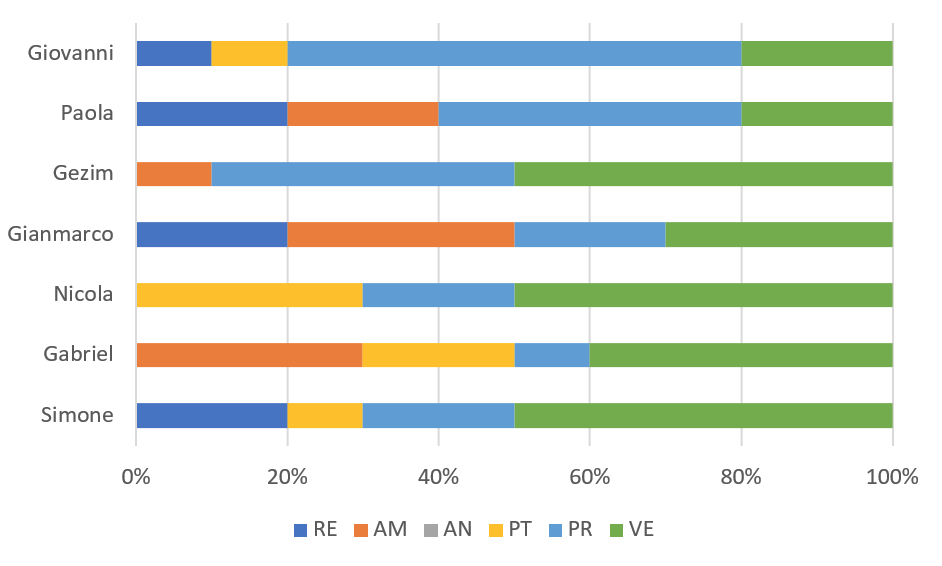
\includegraphics[width=\textwidth]{res/img/hi5}
\
\subsubsection{Prospetto economico}
In abase alle ore necessarie per il completamento di questa fase, il valore economico totale è di 3.128,00 EUR.
\begin{center}
\begin{tabular}{ |c|c|c|  }
 \hline
 Ruolo 		& Ammontare ore 	& Totale (EUR)\\
 	\hline
 \hline
 	Responsabile	& 14 	& 420\\
	Amministratore	& 18		& 360\\
	Analista		& 0 		& 0\\
	Progettista		& 14		& 308\\
	Programmatore	& 42		& 1260\\
	Verificatore	& 52 	& 780\\
 \hline\hline
 TOTALE		& 140		& 3128\\
  \hline
\end{tabular}
\end{center}

\newpage
\subsection{Riepilogo}
\subsubsection{Prospetto orario}
Il team ha previsto la seguente spartizione di ruoli per il completamento del progetto:
\\
\begin{center}
\begin{tabular}{ |c|c|c|c|c|c|c|c|  }
 \hline
 Membro 		& RE 		& AM 		& AN 	& PT 	& PR 	& VE 	& Tot.\\
 \hline\hline
 Simone			& 13 		& 16			& 23 		& 24 		& 33 		& 26 		& 135\\
 Gabriel		& 8 			& 13 		& 22 		& 28		& 40 		& 24 		& 135\\
 Nicola			& 11 		& 14 		& 16 		& 20 		& 29 		& 40 		& 135\\
 Gianmarco		& 12 		& 16 		& 18 		& 27	 	& 34 		& 28 		& 135\\
 Gezim			& 11 		& 18 		& 18 		& 19 		& 36 		& 33	 	& 135\\
 Paola			& 15 		& 12 		& 24 		& 26 		& 28 		& 30 		& 135\\
 Giovanni		& 13 		& 17	 		& 16 		& 17 		& 41	 	& 31  		& 135\\
 \hline\hline
 Ore totali		& 83 	& 106		& 137 	& 161 	& 241 	& 212 	& 940\\
  \hline
\end{tabular}
\end{center}

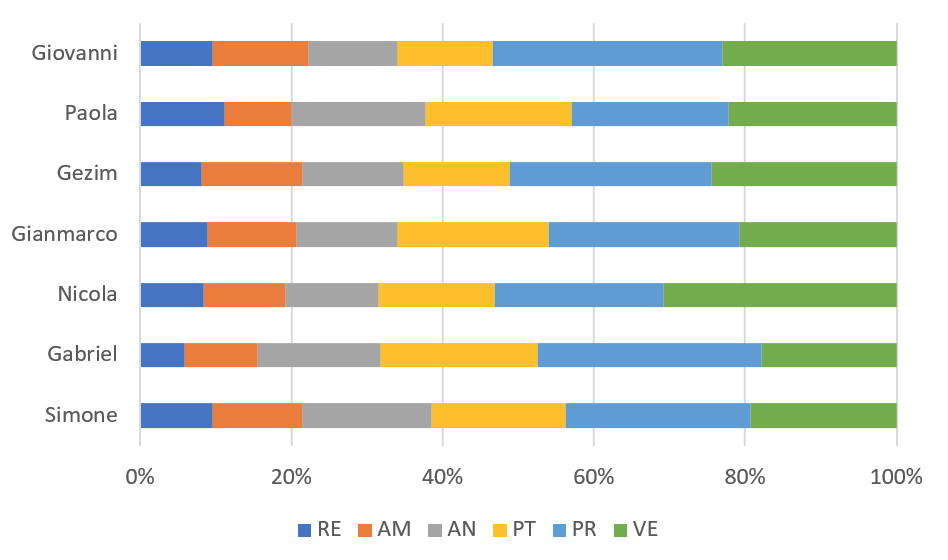
\includegraphics[width=\textwidth]{res/img/hip}
\
\subsubsection{Prospetto economico}
In abase alle ore necessarie per il completamento di questo progetto, il valore economico totale è di 21.987,00 EUR.
\begin{center}
\begin{tabular}{ |c|c|c|  }
 \hline
 Ruolo 		& Ammontare ore 	& Totale (EUR)\\
 	\hline
 \hline
 	Responsabile	& 83 	& 2490\\
	Amministratore	& 106		& 2120\\
	Analista		& 137 		& 3425\\
	Progettista		& 161		& 3542\\
	Programmatore	& 241		& 7230\\
	Verificatore	& 212 	& 3180\\
 \hline\hline
 TOTALE		& 940		& 21987\\
  \hline
\end{tabular}
\end{center}

\subsubsection{Conclusioni}
Il valore economico del progetto è di 21987 EUR. Tuttavia a questo totale bisogna sottrarre il corrispettivo delle fasi \textit{Analisi (4.700,00 EUR)} e \textit{Presentazione (770,00 EUR)} in quanto tali fasi non producono valore per il committente.
\newline
\newline
In conclusione, il totale preventivato per la realizzazione del progetto \textit{Etherless} è di\\ \textbf{16.517,00 EUR}.